\begin{center}

\justifying
\chapter{\large PROJECT IMPLEMENTATION AND CODING}
%\begin{flushleft}
\justifying

\section{\normalsize DATABASE IMPLEMENTATION }
\hspace{1cm}The database used in this project is as given below. It gives information about the tables and their attributes.\\
\hspace*{0.7cm}\textbf{1.Source} 
\\ \hspace*{1cm}src - varchar2 - Primary Key \\

\vspace{0.2in}
\textbf{2.Map} 
\\\hspace*{1cm}src - varchar2 - Foreign Key \\
\hspace*{1cm}src name - varchar2 \\

\vspace{0.2in}
\textbf{3.Flatgraph}
\\ \hspace*{1cm}src -varchar2 - Foreign Key \\
\hspace*{1cm}dest - varchar2 \\
\hspace*{1cm}wt -float \\
\hspace*{1cm}fragid - number\\

\vspace{0.2in}
\textbf{4.frag} 
\\ \hspace*{1cm}fragid - number\\
\hspace*{1cm}src - varchar2 - Foreign Key \\
 \hspace*{1cm}hop - varchar2\\
\hspace*{1cm}wt - float  \\
\hspace*{1cm}bor - number\\

\vspace{0.2in}
\textbf{5.Supergraph} 
\\ \hspace*{1cm}src - varchar2 - Foreign Key \\
\hspace*{1cm}dests - varchar2\\
\hspace*{1cm}hops - varchar2 \\
\hspace*{1cm}wts - float \\
\hspace*{1cm}fragid - number\\

\vspace{0.2in}
\textbf{6.Login} 
\\ \hspace*{1cm}Username -varchar2- Primary Key \\
\hspace*{1cm}Password - varchar2\\
\hspace*{1cm}adminflag - number \\



\section{\normalsize GUI IMPLEMENTATION}
\begin{figure}[H]
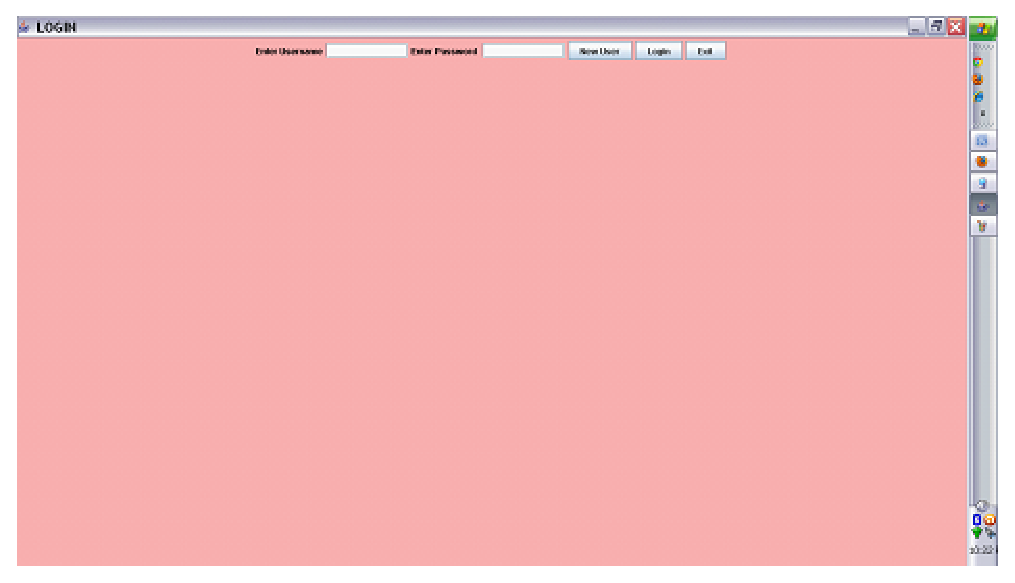
\includegraphics[width=16cm,height=13cm]{login.eps}
\caption{Login Form}
\end{figure}

\begin{figure}[H]
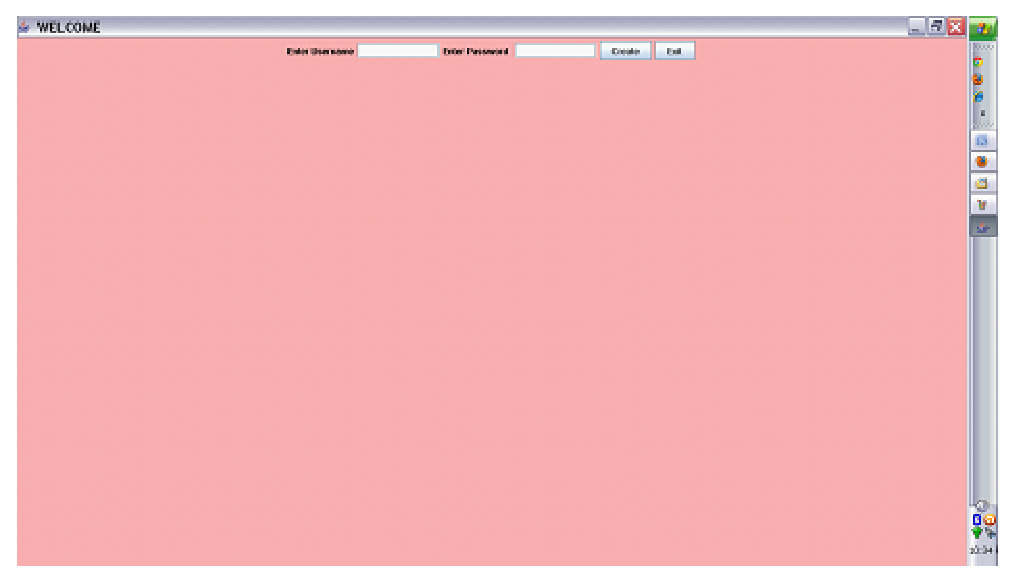
\includegraphics[width=16cm,height=13cm]{newuser.eps}
\caption{New user form}
\end{figure}

\begin{figure}[H]
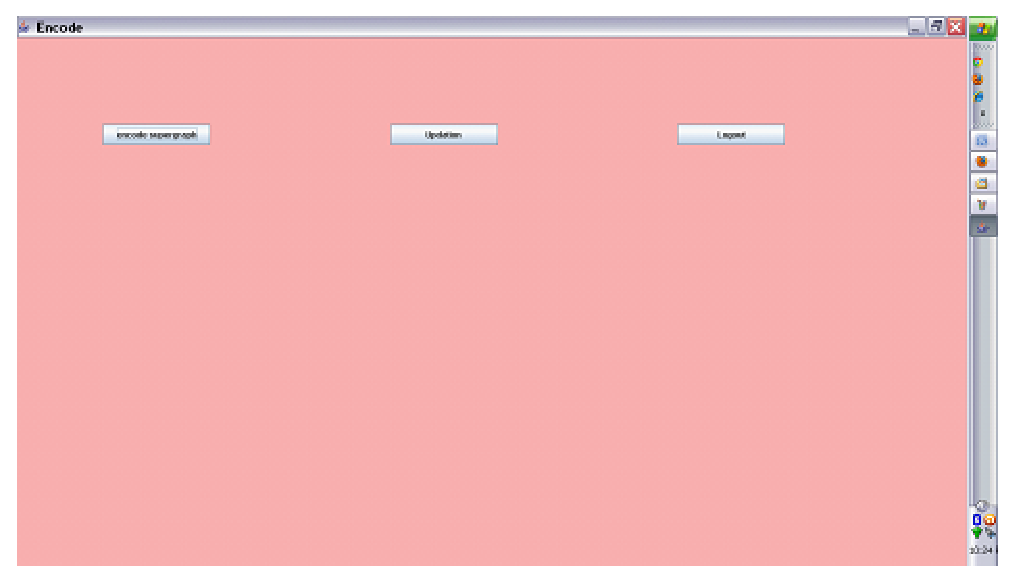
\includegraphics[width=16cm,height=13cm]{admin.eps}
\caption{Admin form}
\end{figure}

\begin{figure}[H]
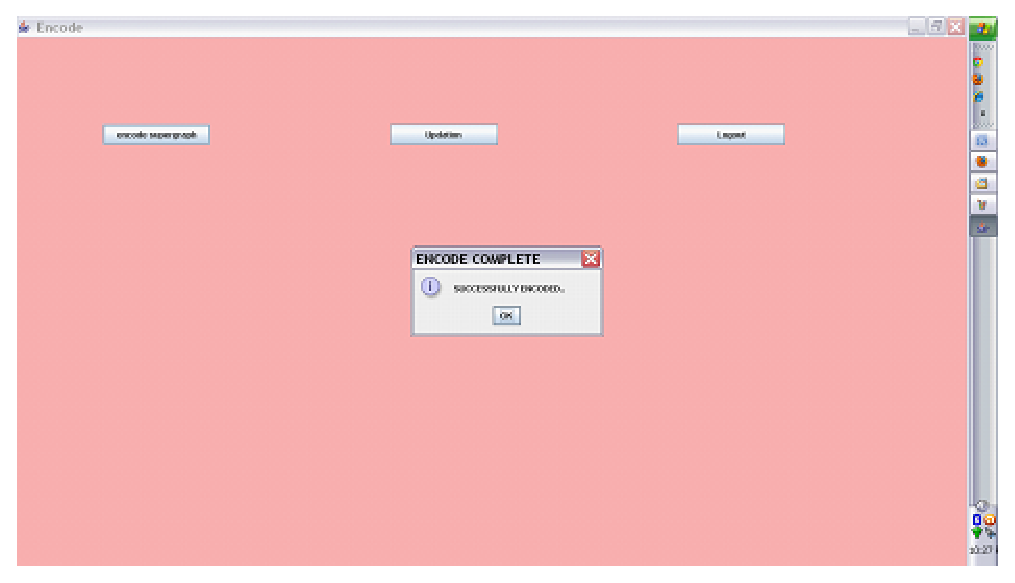
\includegraphics[width=16cm,height=13cm]{encode.eps}
\caption{Encode Form}
\end{figure}

\begin{figure}[H]
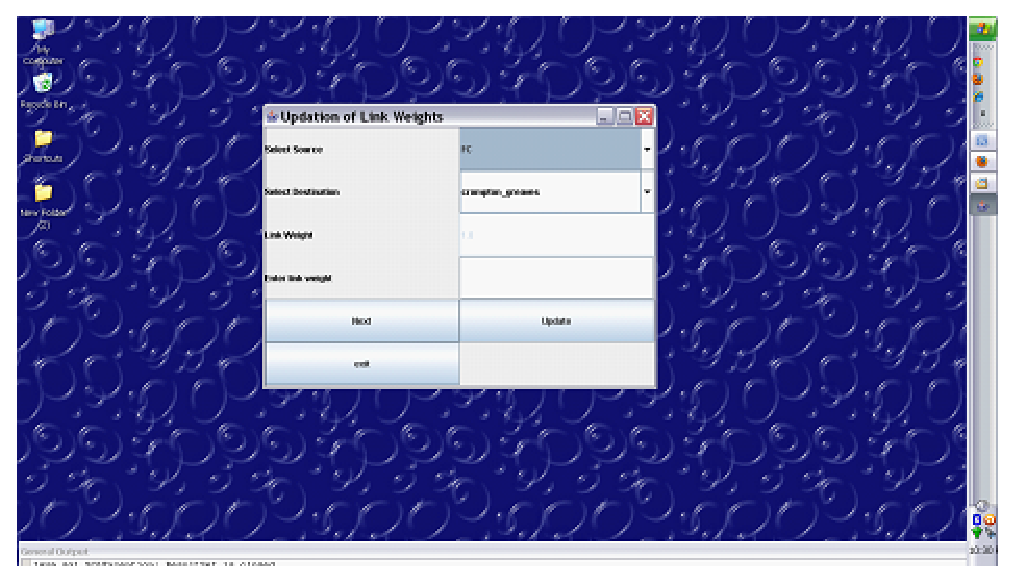
\includegraphics[width=16cm,height=13cm]{update.eps}
\caption{Update Form}
\end{figure}

\begin{figure}[H]
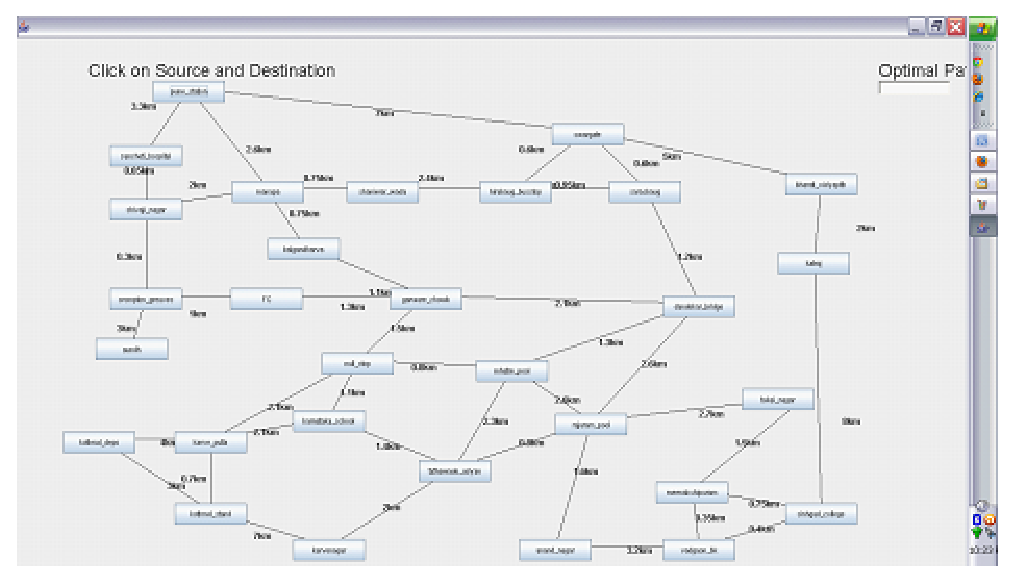
\includegraphics[width=16cm,height=13cm]{map.eps}
\caption{Map Form}
\end{figure}

\begin{figure}[H]
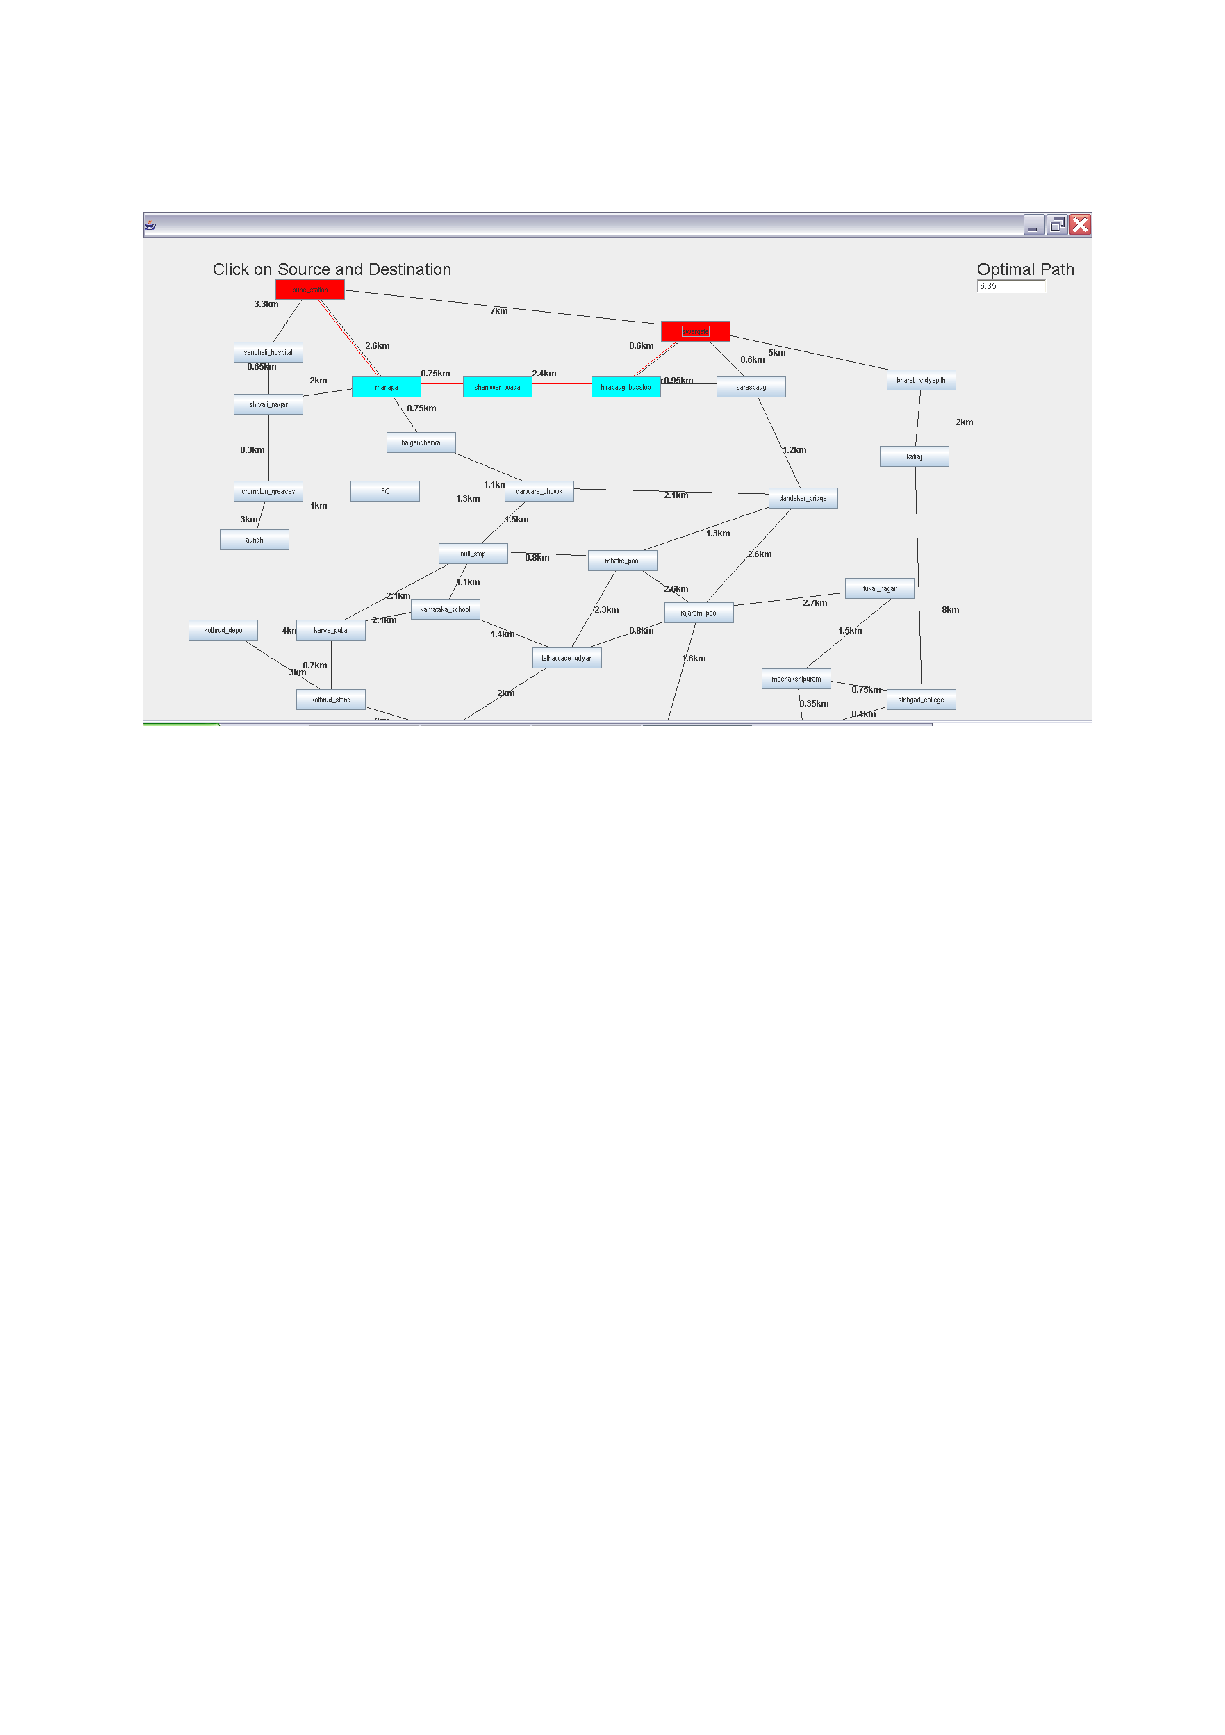
\includegraphics[width=16cm,height=36cm]{mop.eps}
\caption{Map output Form}
\end{figure}

\newpage
\section{\normalsize CODE DETAILS}
\begin{verbatim}
import java.sql.*;
import java.util.*;
import java.io.*;
import javax.swing.*;

class HEPV10
{
	private String superborder[], border[];
	int n,p,l;

	public HEPV10()
	{
		try
		{
			Class.forName("sun.jdbc.odbc.JdbcOdbcDriver");
			Connection con = DriverManager.getConnection("jdbc:odbc:HEPV","system","system");
			Statement st = con.createStatement();
			ResultSet rs = null;

			rs = st.executeQuery("select count(src) from source");	// src is primary key ...
			
			if(rs.next())
				n = rs.getInt("count(src)");
			rs.close();

			rs =st.executeQuery("select count(distinct fragid) from flat_graph");
			if(rs.next())
				p = rs.getInt("count(distinctfragid)");
			rs.close();

			rs = st.executeQuery("select count(*) from flat_graph");
			if(rs.next())
				l = rs.getInt("count(*)");
			rs.close();

			st.close();
			con.close();
		}
		catch(Exception e)
		{
			e.printStackTrace();
		}
		superborder = new String[15];
		border = new String[10];
	}

	public static void main(String[] args)
	{
		JFrame frame = new Map1("Map");
		frame.setVisible(true);
		frame.setExtendedState(frame.getExtendedState()|JFrame.MAXIMIZED_BOTH);
	}

	public void createHEPV()
	{
		Fragment frag = new Fragment();
		Supergraph superg = new Supergraph();

		borderSetting();

		for(int k = 1; k <= p; k++)		// k = fragid
		{
			encode(k);

			for(int c = 0;border[c] != null ;c++)
				border[c] = null;

			bordern(border,k);

			for(int i = 0;border[i]!=null;i++)		// border[i] = src
			{
				for(int j = 0;border[j]!=null;j++)	// border[j] = dest
				{
					if(i != j)
					{
						frag.set(border[i], border[j], k);
						superg.set(border[i], border[j],k);

						float swt, fwt;
						String fhop;

						swt = superg.getWt();
						fwt = frag.getWt();
						fhop = frag.getHop();

						if(fwt < 999.00f)
						{
							if(swt < 999.00f)
							{
								if(swt > fwt)
								{
									superg.update(fhop, fwt);
									System.out.println(" update");
								}
							}
							else
							{
								superg.insert(fhop, fwt);
								System.out.println(" insert");
							}
						}
					}
				}
			}
		}
		encode(0);	// encode supergraph
	}

	public float pathRetrieval(String src,String dest, Map1 frame)
	{
		float SPW = 999.00f;
		int flags = 0, flagd = 0;
		Fragment frag = new Fragment();
		Supergraph superg = new Supergraph();

		if(!src.equals(dest))
		{
			if(superborder[0] == null)
			{
				fillSuperborder();
			}
			for(int i = 0; superborder[i] != null; i++)
			{
				if(superborder[i].equals(src))
				{
					flags = 1; 	// src is a border node (in supergraph)
				}
				else if(superborder[i].equals(dest))
				{
					flagd = 1;	// dest is a border node (in supergraph)
				}
			}
			if(flags == 1 && flagd == 1)		// Case 1: Both src and dest nodes 
			//are border nodes (in supergraph)
			{
				try
				{
					Class.forName("sun.jdbc.odbc.JdbcOdbcDriver");
					Connection con = null;
					ResultSet rs = null;
					ResultSet rs1 = null;
					con = DriverManager.getConnection("jdbc:odbc:HEPV","system","system");
					Statement st = con.createStatement();
					rs1 = st.executeQuery("select * from super_graph 
					where src = '"+ src + "'
					and dests = '"+ dest +"'");

					if(rs1.next())
					{
						SPW = rs1.getFloat("wts");
						String hops = rs1.getString("hops");
						int fragidd = rs1.getInt("fragid");

						System.out.print(src + " -> " + hops);

						frame.highlight(src);	// colour buttons
						frame.highlight(hops);

						int fragids = 0,flag = 1;
						String hopd = null;

						rs = st.executeQuery("select fragid from frag where src  = " + src + " 
						and dest = " + hops + " and wt = (select min(wt) from frag 
						where src = " + src + " and dest = " + hops +")");

						if(rs.next())
						{
							fragids = rs.getInt("fragid");
							bordern(border, fragids);		// border[] is used for src
						}
						rs.close();

						if(fragids == fragidd && fragids != 0)	// src and dest are in same fragment
						{
							while(!hops.equals(dest))
							{
								frag.set(hops,dest,fragids);
								hops = frag.getHop();
								System.out.print(" -> " + hops);
								frame.highlight(hops);
							}
						}
						else		// traverse more than one fragment
						{
							int fragid = 0,indxs = 0;
							float min = 999.0f,wt;
							String hop = null;

							for(int i = 0;i < border.length;i++)
							{
								if(src.equals(border[i]) == false)
								{
									frag.set(hops,border[i],fragids);
									wt = frag.getWt();
									if(min > wt)
									{
										min = wt;
										indxs = i;
										hop = frag.getHop();	// hops -> hop -> border[i]
									}
								}
							}
							if(hop.equals(null) == false)
							{
								System.out.print(" -> " + hop);		// hops -> hop -> border[indxs]
								frame.highlight(hop);
								while(hop.equals(border[indxs]) == false)
								{
									frag.set(hop,border[indxs],fragids);
									hop = frag.getHop();
									System.out.print(" -> " + hop);
									frame.highlight(hop);
								}
							}
							else
							{
								System.out.print(" -> " + border[indxs]);
								frame.highlight(border[indxs]);
							}
							String[] borderd = new String[10];	// border -> borderd
							bordern(borderd, fragidd);	// borderd is used for dest
							min = 999.0f;
							int indxd = 0;
							for(int i = 0;i < borderd.length;i++)
							{
								if(border[indxs].equals(src) == false)
								{
									if(border[indxs].equals(borderd[i]))	
									// if we get same border node in fragids and fragidd
									{
										indxd = i;
										break;
									}
									else
									{
										rs = st.executeQuery("select fragid from super_graph
										where src = " + border[indxs] + " and dests = " + borderd[i]);
										if(rs.next())
											fragid = rs.getInt("fragid");
										frag.set(border[indxs],borderd[i],fragid);
										wt = frag.getWt();
										if(min > wt)
										{
											min = wt;
											hop = frag.getHop();
											indxd = i;
										}
										rs.close();
									}
								}
							}
							if(border[indxs].equals(borderd[indxd]) == false)	
							// 2 different border nodes in different fragment
							{
								while(!hop.equals(borderd[indxd]))
								{
									frag.set(hop,borderd[indxd],fragid);
									hop = frag.getHop();
									System.out.print(" -> " + hop);
									frame.highlight(hop);
								}
							}
							hopd = borderd[indxd];
							while(!hopd.equals(dest))
							{
								frag.set(hopd,dest,fragidd);
								hopd = frag.getHop();
								System.out.print(" -> " + hopd);
								frame.highlight(hopd);
							}
						}
					}
					else
						SPW = 999.0f;
					st.close();
					con.close();
				}
				catch(Exception e)
				{
					System.out.println(e);
				}
			}
			else if(flags == 1 && flagd == 0)	// Case 2: The src is a border node
			//, but the dest is a local node (in fragment)
			{
				try
				{
					Class.forName("sun.jdbc.odbc.JdbcOdbcDriver");
					Connection con = null;
					ResultSet rs = null;
					ResultSet rs1 = null;
					ResultSet rs2 = null;
					con = DriverManager.getConnection("jdbc:odbc:HEPV","system","system");
					Statement st = con.createStatement();
					rs = st.executeQuery("select * from super_graph 
					where src = '" + src + "'");
					if(rs.next())
					{
						int fragids = 0,fragidd = 0;
						String hop = null;

						for(int j = 1;j <= p;j++)
						{
							rs1 = st.executeQuery("select * from frag 
							where fragid = " + j + " and dest = " + dest + " and bor = 0");
							if(rs1.next())
							{
								fragidd = j;
								bordern(border, fragidd);

								float swt = 0.00f,fwt = 0.00f;

								for(int k = 0; border[k]!= null; k++)
								{
									superg.set(src,border[k],0);
									frag.set(border[k],dest,fragidd);

									swt = superg.getWt();
									fwt = frag.getWt();

									if((swt + fwt) < SPW)
									{
										hop = border[k];
										rs2 = st.executeQuery("select fragid from super_graph 
										where src  = '" + src + "' and dests = '" + border[k] + "'");
										if(rs2.next())
										{
											fragids = rs2.getInt("fragid");
										}
										rs2.close();
										SPW = swt + fwt;
									}
								}
								System.out.print(src);
								frame.highlight(src);
								while(!src.equals(hop))
								{
									frag.set(src,hop,fragids);
									src = frag.getHop();
									System.out.print(" -> " + src);
									frame.highlight(src);
								}
								while(!hop.equals(dest))
								{
									frag.set(hop,dest,fragidd);
									hop = frag.getHop();
									System.out.print(" -> " + hop);
									frame.highlight(hop);
								}
								rs1.close();
								break;
							}
						}
					}
					rs.close();
					st.close();
					con.close();
				} //try
				catch(Exception e)
				{
					System.out.println(e);
				}
			}
			
			else		// Case 3: Both the src and dest nodes are local nodes (in fragment)
			{
				try
				{
					int flag = 0;
					String hops = null,hopd = null;

					Class.forName("sun.jdbc.odbc.JdbcOdbcDriver");
					Connection con = null;
					ResultSet rs = null;
					ResultSet rs1 = null;
					con = DriverManager.getConnection("jdbc:odbc:HEPV","system","system");
					Statement st = con.createStatement();
					int fragids = 0,fragidd = 0;

					for(int i = 1; i <= p; i++)
					{
		rs = st.executeQuery("select * from frag 
		where fragid = " + i + " and src = '" + src + "'");
						if(rs.next())
						{
							bordern(border, i);		// border[] is used for src
							fragids = i;
							rs.close();
							break;
						}
						rs.close();
					}
					String[] borderd = new String[10];
					for(int j = 1; j <= p; j++)
					{
		rs = st.executeQuery("select * from frag 
		where fragid = " + j + " and dest = '" + dest + "'");
						if(rs.next())
						{
							bordern(borderd, j);	// borderd is used for dest
							fragidd = j;
							rs.close();
							break;
						}
						rs.close();
					}
					if(fragids!=0 && fragidd!=0)
					{
						float swt,fwts,fwtd;

						for(int i = 0; border[i]!= null; i++)
						{
							for(int j = 0; borderd[j]!=null; j++)
							{
								frag.set(src,border[i],fragids);
								fwts = frag.getWt();
								superg.set(border[i],borderd[j],0);
								swt = superg.getWt();
								frag.set(borderd[j], dest,fragidd);
								fwtd = frag.getWt();
								if((swt + fwts + fwtd) < SPW)
								{
									hops = border[i];
									hopd = borderd[j];
									SPW = swt + fwts + fwtd;
									flag = 1;
								}
							}
						}
					}
					if(fragids == fragidd && fragids != 0)
					{
						float fwt;

						frag.set(src,dest,fragids);
						fwt = frag.getWt();
						if(fwt < SPW)
						{
							hops = frag.getHop();
							SPW = fwt;
							flag = 2;
						}
					}
					if(flag == 1)
					{
						int fragid = 0;

						System.out.print(src);
						frame.highlight(src);

						while(!src.equals(hops))
						{
							frag.set(src,hops,fragids);
							src = frag.getHop();
							System.out.print(" -> " + src);
							frame.highlight(src);
						}

						rs = st.executeQuery("select fragid from super_graph 
						where src = '" + hops + "' and dests = '" + hopd + "'");
						if(rs.next())
						{
							fragid = rs.getInt("fragid");
						}

						while(!hops.equals(hopd))
						{
							frag.set(hops,hopd,fragid);
							hops = frag.getHop();
							System.out.print(" -> " + hops);
							frame.highlight(hops);
						}

						while(!hopd.equals(dest))
						{
							frag.set(hopd,dest,fragidd);
							hopd = frag.getHop();
							System.out.print(" -> " + hopd);
							frame.highlight(hopd);
						}
					}
					else if(flag == 2)
					{
						System.out.print(src + " -> " + hops);
						frame.highlight(src);
						frame.highlight(hops);

						while(!hops.equals(dest))
						{
							frag.set(hops,dest,fragids);
							hops = frag.getHop();
							System.out.print(" -> " + hops);
							frame.highlight(hops);
						}
					}

					rs.close();
					st.close();
					con.close();
				} //try
				catch(Exception e)
				{
					System.out.println(e);
				}
			}
		}
		else
System.out.println("Source and Destination are same. Thus, shortest distance = 0.0");

		return SPW;
	}
	private int flatUpdate(String src, String dest,float linkwt)
	{
		int fragid = 0;

		try
		{
			Class.forName("sun.jdbc.odbc.JdbcOdbcDriver");
			Connection con = null;
			ResultSet rs = null;
			con = DriverManager.getConnection("jdbc:odbc:HEPV","system","system");
			Statement st = con.createStatement();
st.executeUpdate("Update flat_graph set wt = " + linkwt + " 
where src = '" + src + "' and dest = '" + dest + "'");
rs = st.executeQuery("select fragid from flat_graph 
where src = '" + src + "' and dest = '" + dest + "'");
			if(rs.next())
			{
				fragid = rs.getInt("fragid");
			}
			rs.close();

			st.close();
			con.close();
		}
		catch(Exception e)
		{
			System.out.println(e);
		}
		return fragid;
	}

	public void HEPVUpdate()
	{
		int fragid[] = new int[p];
		String ch, borderc[] = new String[10], bor[] = new String[10];

		for(int i = 0; i < p; i++)
			fragid[i] = 0;

		do
		{
			Scanner sc = new Scanner(System.in);

			System.out.println("Enter src: \t");
			String src = sc.nextLine();

			System.out.println("Enter dest: \t");
			String dest = sc.nextLine();

			System.out.println("Enter new linkwt:\t");
			float linkwt = Float.parseFloat(sc.nextLine());

			int id = flatUpdate(src,dest,linkwt);
			fragid[--id] = 1;

			System.out.println("Do you want change any links?");
			ch = sc.nextLine();

		}while(ch == "y");


		for(int i = 0; i < p; i++)
		{
			if(fragid[i] == 1)
				encode(i+1);
		}


		for(int i = 0; border[i]!= null; i++)
		{
			border[i] = null;
			borderc[i] = null;
		}

		for(int i = 0; i < p; i++)
		{
			if(fragid[i] == 1)
			{
				bordern(border,i+1);

				for(int j = 0; border[j] != null; j++)
				{
					for(int k = 0; border[k] != null; k++)
					{
						if(j != k)
						{
							Supergraph superg = new Supergraph();
							superg.set(border[j], border[k], i+1);
							superg.update(null,999.00f);
						}
					}
				}
			}
		}

		for(int k = 1; k <= p; k++)
		{
			for(int i = 0; border[i]!=null; i++)
			{
				border[i] = null;
			}
			bordern(border,k);

			for(int l = 0; l < p; l++)
			{
				if(fragid[l] == 1)
				{
					for(int i = 0; borderc[i] != null; i++)
					{
						borderc[i] = null;
					}
					bordern(borderc,l+1);

					int c = 0;

					for(int u =0; border[u] != null;u++) 
					// create bor[] for Ni, Nj that belong to both //border[] and borderc[]
					{
						for(int v = 0; borderc[v] != null;v++)
						{
							if(border[u] == borderc[v])
							{
								int i;
								for(i = 0; bor[i] != null; i++) // no duplicate entries
								{
									if(bor[i] == border[u])
										break;
								}
								if(bor[i] == null)
									bor[c++] = border[u];
							}
						}
					}

					for(int i = 0; bor[i] != null; i++)
					{
						for(int j = 0; bor[j] != null; j++)
						{
							if(bor[i] != bor[j])
							{
								Supergraph superg = new Supergraph();
								Fragment frag = new Fragment();

								superg.set(bor[i], bor[j], l+1);
								frag.set(bor[i], bor[j], l+1);

								float fwt = frag.getWt();
								float swt = superg.getWt();

								if(fwt < 999.00f && swt > fwt)
								{
									superg.update(frag.getHop(),fwt);
								}
							}
						} // for j
					} // for i
				}
			} // for l
		} // for k

		encode(0);	// encode supergraph
	}
}
\end{verbatim}






